\chapter{Horn clause solving}
\label{chap:horn}

The problems are generated by encoding constraints over execution
paths with unknown predicates which describe functions' constraints
between parameters and return values.



We propose a new algorithm for solving recursion-less Horn clauses to
generate a solution which is as simple as possible.  This enables us
to obtain appropriate predicates that are suitable for predicate
abstraction in the program verification techniques.

The construction of the algorithm roughly consists of two parts.
\begin{itemize}
\item \textbf{Iterative Constraint Generation} is a process to build a
  constraint to compute a solution.  It starts from generating the
  weakest constraint in the sense that the resulting solution would
  not be simple yet.  The process iteratively strengthens a constraint
  until the strongest one while preserving the constraint
  satisfiability.  The strongest constraint gives a simple solution.
\item \textbf{Problem Restructuring} is a process to restructure the
  problem to obtain a less simple solution, if the constraint become
  unsatisfiable during the iterative constraint generation.  This
  process considers the unsatisfiable core of the constraint, and
  wisely enlarges the solution size.
\end{itemize}

All predicate variables in an input problem are assigned simple
templates.  Those predicate templates are parameterized.  In the
iterative constraint generation process, algorithm builds a linear
constraint that parameters in templates must satisfy.  This is done in
a constructive manner, and constraints are built in the order of
implication dependency in Horn clauses.  That is, when an input
problem has a Horn clause that has a predicate variable $P$ on its
left-hand and $Q$ on its right-hand, a constraint to describe
parameters in $P$'s template are first build before those in $Q$'s
template.  When all parameters in the whole problem are described, the
built constraint is evaluated to obtain a model.  Its instantiation
becomes an appropriate solution for the input problem.

The novelty of our algorithm lies in the incremental constraint
refinement.  The algorithm tries to solve from the weakest constraint
that an input problem allows that does not give a simple solution, and
gradually strengthen the constraint until it reaches to the simplest
solution that the problem has.  When a constraint becomes
unsatisfiable during this step, the algorithm analyzes the
unsatisfiable core and transforms the problem to obtain a less simple
solution.

This construction of the algorithm enables us to compute a relatively
simpler solution compared to existing algorithms while restraining the
computation cost in a reasonable time.

\section{Example}

\begin{figure}
\begin{center}
\includegraphics[scale=0.8]{figures/ex1.eps}
\end{center}
\vspace{-18pt}
\caption{Problem visualization for tree interpolation example}
\label{fig:ex1}
\end{figure}

\paragraph {Tree interpolation}
First, consider the following example.
\begin{align*}
x \leq 1 & \implies A(x) \\
y \leq 2 & \implies B(y) \\
A(x) \wedge B(y) & \implies 3x+2y \leq 10
\end{align*}
In this example, we would like to compute linear arithmetic formulas
for the predicate variables $A$ and $B$.  They appear only once on
both left-hand and right-hand globally in the problem.  For ease of
understanding, we visualized the problem by a graph in Figure~\ref{fig:ex1}.

We try to obtain a simple solution that is expressed by linear
expression templates, whose coefficients and constants are
parameterized.  Assume that they have following predicate templates.
\begin{align*}
A(x) : c_1 x + c_2 \leq 0 \\
B(y) : c_3 y + c_4 \leq 0
\end{align*}

By naturally encoding the first Horn clause with Farkas's lemma, we
obtain a linear constraint
$(\lambda_1 = c_1) \wedge (- \lambda_1 \geq c_2) \wedge (\lambda_1 \geq 0)$.
Any assignment to $ c_1, c_2, \lambda_1 $ which satisfies this will
make $A(x)$ valid for the first clause.  In the same manner, we obtain
$(\lambda_2 = c_3) \wedge (- 2 \lambda_2 \geq c_4) \wedge (\lambda_2 \geq 0)$
from the second clause, and 
$(c_1 = 3 \lambda_3) \wedge (c_3 = 2 \lambda_3) \wedge (c_2 + c_4 \geq -10 \lambda_3) \wedge (\lambda_3 > 0)$
from the third.

One of the models satisfying all the constraints above is
\[( c_1, c_2, c_3, c_4, \lambda_1, \lambda_2, \lambda_3 ) = (3, -3, 2, -4, 3, 2, 1) \].
By assigning them to the template, we obtain the following solution.
\begin{align*}
A(x) : 3 x - 3 \leq 0 \\
B(y) : 2 y - 4 \leq 0
\end{align*}

\paragraph {DAG problem solving}

\begin{figure}
\begin{center}
\includegraphics[scale=0.8]{figures/ex2-1.eps}
\end{center}
\caption{Problem visualization for DAG structured example}
\label{fig:ex21}
\end{figure}

Second, we explain a case that some predicate variables appear
multiple times on left-hand side in different Horn clauses.
\begin{align*}
x \leq 1 & \implies A(x) \\
A(x) \wedge A(y) & \implies x+y \leq 2
\end{align*}
Problem visualization is available in Figure~\ref{fig:ex21}. Note
that the graph now takes a DAG structure.

Assigning a template $A(x) : c_1 x + c_2 \leq 0$, we obtain the same
constraint for the first clause as the previous example.
\begin{align} \label{eq:constr1}
(\lambda_1 = c_1) \wedge (- \lambda_1 \geq c_2) \wedge (\lambda_1 \geq 0)
\end{align}

Since we have $A$'s appearance twice on the second clause, it is
possible for $A$ to have two expressions each of which is used for
$A(x)$ and $A(y)$.  Although we need to use the same template for
multiple occurrences in order to compute the simplest solution, it may
generally make the whole constraints unsatisfiable if the simplest
solution does not exist.

The above case eventually generate the constraint
\begin{align*}
& (\lambda_1 = c_1) \wedge (- \lambda_1 \geq c_2) \wedge (\lambda_1 \geq 0) \wedge \\
& (c_1 = \lambda_2) \wedge (2 c_2 \geq 2 \lambda_2) \wedge (\lambda_2 > 0)
\end{align*}
and we may get a model $(c_1, c_2, \lambda_1) = (1, -1, 1)$ to
obtain $Ax - 1 \leq 0$ for $A(x)$.

\begin{figure}[htb]
  \begin{minipage}[t]{.47\textwidth}
  \centering
  \includegraphics[scale=0.8]{figures/ex2-2.eps}
  \caption{Modified problem}
  \label{fig:ex22}
  \end{minipage}
  \hfill
  \begin{minipage}[t]{.47\textwidth}
  \centering
  \includegraphics[scale=0.8]{figures/ex2-3.eps}
  \caption{Problem transformation}
  \label{fig:ex23}
  \end{minipage}
\end{figure}

Now we slightly change the problem.
\begin{align*}
x \leq 1 & \implies A(x) \\
A(x) \wedge A(y) & \implies x+2y \leq 3
\end{align*}
It is visualized in Figure~\ref{fig:ex22}.  The modifed constraint is
\begin{align*}
& (\lambda_1 = c_1) \wedge (- \lambda_1 \geq c_2) \wedge (\lambda_1 \geq 0) \wedge \\
& (c_1 = \lambda_2) \wedge (c_1 = 2\lambda_2) \wedge (2 c_2 \geq 3 \lambda_2) \wedge (\lambda_2 > 0)
\end{align*}
No solution exists for this constraint.  Therefore we generate a
weaker constraint for the second clause that allows different
expressions of $A$ for multiple occurrence.  If the whole constraint
is satisfiable in the case, we try to solve in a stronger constraint
to generate a simple solution.

In this specific case, it is virtually equivalent to solve the
following problem in a weaker constraint.
\begin{align*}
\text{Problem:} \\
x \leq 1 & \implies A_1(x) \\
x \leq 1 & \implies A_2(x) \\
A_1(x) \wedge A_2(y) & \implies x+y \leq 2 \\
\\
\text{Templates:} \\
A_1(x) \text{ : } & c_{1,1} x + c_{2,1} \leq 0 \\
A_2(x) \text{ : } & c_{1,2} x + c_{2,2} \leq 0 \\
A(x) \text{ : } & A_1(x) \wedge A_2(x) \\
\end{align*}
Figure~\ref{fig:ex23} illustrates above.  By duplicating the
constraint~\ref{eq:constr1} of $A$ for newly created $A_1$ and $A_2$,
we obtain the whole constraint as follows.
\begin{align*}
& \lambda_{1,1} = c_{1,1} \wedge - \lambda_{1,1} \geq c_{2,1} \wedge \lambda_{1,1} \geq 0 \wedge \\
& \lambda_{1,2} = c_{1,2} \wedge - \lambda_{1,2} \geq c_{2,2} \wedge \lambda_{1,2} \geq 0 \wedge \\
& c_{1,1} = \lambda_2 \wedge c_{1,2} = \lambda_2 \wedge c_{2,1} + c_{2,2} \geq 2 \lambda_2 \wedge \lambda_2 > 0
\end{align*}

This constraint is satisfiable and one model is
\[ ( c_{1,1}, c_{1,2}, c_{2,1}, c_{2,2}, \lambda_{1,1}, \lambda_{1,2}, \lambda_2 ) =
( 1, -1, 1, -1, 1, 1, 1 ) \] and the solution then becomes
$A(x) : (x -1 \leq 0) \wedge (x -1 \leq 0)$.

Since the weak constraint is satisfiable, we now refine the constraint
to obtain the better solution.  That is, simply eliminate the
duplication to build the following constraint for the original
template.

\begin{align*}
& \lambda_1 = c_1 \wedge - \lambda_1 \geq c_2 \wedge \lambda_1 \geq 0 \wedge \\
& c_1 = \lambda_2 \wedge c_1 = \lambda_2 \wedge 2 c_2 \geq 2 \lambda_2 \wedge \lambda_2 > 0
\end{align*}

Solving this constraint simply gives us a solution
$A(x) : x -1 \leq 0$.

\paragraph {Disjunctive Horn clause solving}
Finally, we explain a case that an input set of Horn clauses contain
disjunctions on left-hand side.
\begin{figure}
  \begin{center}
    \includegraphics[scale=0.8]{figures/ex3-1.eps}
  \end{center}
  \caption{Visualization of disjunctive Horn clause problem}
  \label{fig:ex31}
\end{figure}
\begin{align*}
x \leq 0 \wedge -x \leq 0 & \implies A(x) \\
x+1 \leq 0 \vee -x+1 \leq 0 & \implies B(x) \\
A(x) \wedge B(x) & \implies 1 \leq 0
\end{align*}
See Figure~\ref{fig:ex31}.  Same as the previous examples, templates
for predicate variables are prepared.
\begin{align*}
A(x) : c_1 x + c_2 \leq 0 \\ B(x) : c_3 x + c_4 \leq 0
\end{align*}
The constraints generated are follows.
\begin{align*}
& \lambda_1 - \lambda_2 = c_1 \wedge 0 \geq c_2 \wedge \lambda_1 \geq 0 \wedge \lambda_2 \geq 0 \wedge \\
& \lambda_3 = c_3 \wedge \lambda_3 \geq c_4 \wedge \lambda_3 \geq 0 \wedge \\
& - \lambda_4 = c_3 \wedge \lambda_4 \geq c_4 \wedge \lambda_4 \geq 0 \wedge \\
& c_1 + c_3 = 0 \wedge c_2 + c_4 > 0
\end{align*}
The constraints here become unsatisfiable, and one possible
unsatisfiable core is:
\begin{align*}
\lambda_3 & = c_3 \\
\lambda_3 & \geq c_4 \\
- \lambda_4 & = c_3 \\
\lambda_4 & \geq c_4 \\
c_2 + c_4 & > 0 \\
0 & \geq c_2
\end{align*}

Because the unsatisfiable core contains constraints originating from
the disjunctions to be expressed in a single term template, we can
determine which predicate to relax its template to allow an enlarged solution.

Now we slightly change the problem and the template as in Figure~\ref{fig:ex32}.
\begin{align*}
\text{Problem:} \\
x \leq 0 \wedge -x \leq 0 & \implies A(x) \\
x+1 \leq 0 & \implies B_1(x) \\
-x+1 \leq 0 & \implies B_2(x) \\
A(x) \wedge B_1(x) & \implies 1 \leq 0 \\
A(x) \wedge B_2(x) & \implies 1 \leq 0 \\
\\
\text{Templates:} \\
A(x) \text{ : } & c_1 x + c_2 \leq 0 \\
B_i(x) \text{ : } & c_{3,i} x + c_{4,i} \leq 0 \quad (i \in \left\lbrace 1,2 \right\rbrace ) \\
B(x) \text{ : } & B_1(x) \vee B_2(x)
\end{align*}

\begin{figure}
  \begin{center}
    \includegraphics[scale=0.8]{figures/ex3-2.eps}
  \end{center}
  \caption{First transformation}
  \label{fig:ex32}
\end{figure}
When we construct the constraints, as same as previous, we again
obtain an unsatisfiable core:
\begin{align*}
\text{Constraint:} \\
& \lambda_1 - \lambda_2 = c_1 \wedge 0 \geq c_2 \wedge \lambda_1 \geq 0 \wedge \lambda_2 \geq 0 \wedge \\
& \lambda_3 = c_{3,1} \wedge \lambda_3 \geq c_{4,1} \wedge \lambda_3 \geq 0 \wedge \\
& \lambda_3 = c_{3,2} \wedge \lambda_3 \geq c_{4,2} \wedge \lambda_3 \geq 0 \wedge \\
& - \lambda_4 = c_{3,1} \wedge \lambda_4 \geq c_4 \wedge \lambda_4 \geq 0 \wedge \\
& - \lambda_4 = c_{3,2} \wedge \lambda_4 \geq c_{4,2} \wedge \lambda_4 \geq 0 \wedge \\
& c_1 + c_{3,1} = 0 \wedge c_2 + c_{4,1} > 0 \wedge \\
& c_1 + c_{3,2} = 0 \wedge c_2 + c_{4,2} > 0
\\
\text{Unsatisfiable core:} \\
& 0 \geq c_2 \\
& \lambda_3 = c_{3,1} \\
& \lambda_3 \geq c_{4,1} \\
& - \lambda_4 = c_{3,2} \\
& c_1 + c_{3,1} = 0 \\ & c_2 + c_{4,1} > 0 \\
& c_1 + c_{3,2} = 0
\end{align*}
This time, the unsatisfiable core contains the constraints that
originate from conjunction.  We need to modify the problem again.
\begin{align*}
\text{Problem:} \\
x \leq 0 \wedge -x \leq 0 & \implies A_i(x) \quad (i \in \left\lbrace 1,2 \right\rbrace ) \\
x+1 \leq 0 & \implies B_1(x) \\
-x+1 \leq 0 & \implies B_2(x) \\
A_i(x) \wedge B_j(x) & \implies 1 \leq 0 \quad (i,j \in \left\lbrace 1,2 \right\rbrace ) \\
\\
\text{Templates:} \\
A_i(x) \text{ : } & c_{1,i} x + c_{2,i} \leq 0 \quad (i \in \left\lbrace 1,2 \right\rbrace ) \\
A(x) \text{ : } & A_1(x) \wedge A_2(x) \\
B_i(x) \text{ : } & c_{3,i} x + c_{4,i} \leq 0 \quad (i \in \left\lbrace 1,2 \right\rbrace ) \\
B(x) \text{ : } & B_1(x) \vee B_2(x)
\end{align*}
See Figure~\ref{fig:ex33}.

\begin{figure}
  \begin{center}
    \includegraphics[scale=0.8]{figures/ex3-3.eps}
  \end{center}
  \caption{Second transformation}
  \label{fig:ex33}
\end{figure}

After this, we obtain the following constraint:
\begin{align*}
& \lambda_1 - \lambda_2 = c_{1,1} \wedge 0 \geq c_{2,1} \wedge \lambda_1 \geq 0 \wedge \lambda_2 \geq 0 \wedge \\
& \lambda_1 - \lambda_2 = c_{1,2} \wedge 0 \geq c_{2,2} \wedge \lambda_1 \geq 0 \wedge \lambda_2 \geq 0 \wedge \\
& \lambda_3 = c_{3,1} \wedge \lambda_3 \geq c_{4,1} \wedge \lambda_3 \geq 0 \wedge \\
& \lambda_3 = c_{3,2} \wedge \lambda_3 \geq c_{4,2} \wedge \lambda_3 \geq 0 \wedge \\
& - \lambda_4 = c_{3,1} \wedge \lambda_4 \geq c_4 \wedge \lambda_4 \geq 0 \wedge \\
& - \lambda_4 = c_{3,2} \wedge \lambda_4 \geq c_{4,2} \wedge \lambda_4 \geq 0 \wedge \\
& c_{1,1} + c_{1,2} + c_{3,1} = 0 \wedge c_{2,1} + c_{2,2} + c_{4,1} > 0 \wedge \\
& c_{1,1} + c_{1,2} + c_{3,2} = 0 \wedge c_{2,1} + c_{2,2} + c_{4,2} > 0
\end{align*}
By solving this, we eventually obtain the following solution.
\begin{align*}
A(x) \text{ : } & x \leq 0 \wedge -x \leq 0 \\
B(x) \text{ : } & x+1 \leq 0 \vee -x+1 \leq 0
\end{align*}

\section{Preliminaries}

For ease of discussion, our algorithm handles an input set of Horn
clauses by a \emph{Horn graph} that express the equivalent problem.
The graph is then used throughout the algorithm to represent the
problem.  A Horn graph is a labeled directed acyclic graph
$G=(V,E,\varphi)$.
\begin{itemize}
\item $V$ is a union of two disjoint sets of vertices; Horn term
  vertices $V_T$ and arrow vertices $V_\Rightarrow$.  Each vertex
  $u \in V_\Rightarrow$ has exactly one outgoing edge to some
  $v \in V_T$, denoted as $succ(u)$.
\item $E$ is a set of labeled edges, which are expressed in the form
  $(u,v,\theta)$ where $\theta$ is a finite map from variables to
  variables.
\item $\varphi: V_T \rightarrow L$ is a labeling function for Horn
  term vertices, where L is a set of elements of a predicate variable
  in the form $P(x_1, \ldots, x_{\mathrm{arity}(P)})$ or a linear
  inequality $a_1 x_1 + \cdots + a_n x_n + b \leq 0$.
\end{itemize}
There are two kinds of edges in a Horn graph;
\begin{itemize}
\item for $u \in V_T, v \in V_\Rightarrow$, an edge takes a form
  $(u,v,\theta)$, written $\edgel{u}{\theta}{v}$, or,
\item for $u \in V_\Rightarrow, v \in V_T$, an edge takes a form
  $(u,v,\emptyset)$, written $\edge{u}{v}$, where the mapping is
  empty.
\end{itemize}

We define the relation $\leadsto$ over $V_T$ as follows.
\[ u \mathop{\leadsto}^\theta v \Longleftrightarrow \exists a \in V_\Rightarrow;
\edgel{u}{\theta}{a} \wedge \edge{a}{v} \]
We may omit $\theta$ and write $u \leadsto v$ for convenience in later
discussions. By the assumption that $G$ is acyclic, both
$\rightarrow^+$ and $\leadsto^+$ are well-founded relations. $v_\bot$
is the greatest element with respect to both $\rightarrow^+$ and
$\leadsto^+$.

The meaning $\llbracket G \rrbracket $ of a Horn graph $G$ is a set of
Horn clauses $\mathcal{HC}_v$ for all vertices $v \in V_\Rightarrow$.
\begin{align*}
\mathcal{HC}_v & = \left( \bigwedge_{(u,v,\theta) \in E} \theta \varphi(u) \right) \Longrightarrow \varphi(succ(v)) \\
\llbracket G \rrbracket & = \bigwedge_{v \in V_\Rightarrow} \mathcal{HC}_v
\end{align*}
We implicitly assume each $\mathcal{HC}_v$ is universally quantified
by its all free variables $\textsc{FV}(\mathcal{HC}_v)$.

Horn term vertices with predicate variable labels are unique each
other that any of them do not have the same variable on their labels.
From now on, we may denote a Horn term vertex with a predicate
variable label by its predicate variable name if no ambiguity is
present.

Without loss of generality, we assume the existence of the
\emph{root vertex} $v_\bot \in V_T$ with linear expression labels
$1 \leq 0$, meaning $\bot$.  This is because if we have a Horn clause
$P \implies e$ which $e$ is a linear expression, we can convert it to
$P \wedge \neg e \implies 1 \leq 0$.  We also assume that other
vertices with linear expression labels have no incoming edges to them.

For simplicity of discussion, we define \emph{term arity} $k_v$ for
every Horn term vertex $v \in V_T$ with incoming edges.
\begin{align*}
k_v =
\begin{cases}
\mathrm{arity}(P) & \mbox{if } \varphi(v) = P(x_1,...,x_{\mathrm{arity}(P)}) \\
0 & \mbox{if } \varphi(v) = \bot
\end{cases}
\end{align*}
We let $K$ denote the maximum of $k_v$ over all $v \in V_T$.

A variable mapping label $\theta$ on edges is used to map the index of
one predicate variable to another.

The algorithm assigns a \emph{predicate template} for all predicate
variables in $G$. A \emph{predicate templateset} is a set of mappings
from a predicate variable to a predicate template.  A template for a
predicate variable $P(x_1, \ldots, x_n)$ is a formula $\psi$
constructed from the following definition.
\begin{align*}
\psi ::= & a_1 x_1 + \cdots + a_n x_n + b \leq 0 \mid \\
& \psi \wedge \psi \mid \psi \vee \psi
\end{align*}
A linear expression in the definition above may also be represented in
a equivalent vector form $\mathbf{a} \mathbf{x} + b \leq 0$ for short.
Parameters $\mathbf{a}$ and $b$ are specified by a linear constraint.

The solution of $G$ is a map $\rho$ from predicate variables to linear
predicates of the form $\lambda x_1, \ldots ,x_n. \psi$ where
parameters in $\psi$ are replaced with constant and $\rho[G]$ becomes
a tautology.  A solution is \textit{simple} if $\rho[P]$ is of the
form $\mathbf{a} \mathbf{x} + b \leq 0$ for every $P$ in
$\mathrm{dom}(\rho)$.

The problem of solving Horn clauses (represented by $G$) is to find a
solution of $G$ (and a simple solution if possible).

\section{Simple solution}

We first propose an algorithm to compute a simple solution for the
given Horn graph $G$ if one exists.  Later we add modifications to the
algorithm for the case that a simple solution does not exist for $G$.
In such a case, we transform the input graph $G$ to have a larger
solution template.

For each vertex $v \in V$, we define
$\Delta(v) = (\mathbf{a}_v \mathbf{x}_v + b_v \leq 0, C_v)$
, where
\begin{itemize}
\item $\mathbf{a}_v \mathbf{x}_v + b_v \leq 0$ is a linear inequality
  that contains coefficient variables $\mathbf{a}_v$ and a constant
  $b_v$, and
\item $C_v$ is a set of linear expressions on coefficient variables.
\end{itemize}
Intuitively, it denotes the set of inequalities:
\begin{align*}
\left\lbrace
 \mathbf{a}_v \mathbf{x}_v + b_v \leq 0 \mid
 \exists \left( \textsc{FV}(C_v)
  \setminus (\mathbf{a}_v \cup \left\lbrace b_v \right\rbrace
 \right); C_v
\right\rbrace
\end{align*}
For a predicate variable vertex,
$\mathbf{a}_v \mathbf{x}_v + b_v \leq 0$ serves as a predicate
template and $C_v$ describes the parameters $\mathbf{a}_v$ and $b_v$.

$C_v$ is defined by well-founded induction on $v$ with respect to the
relation $\rightarrow^+$. Then, $C_v$ can be shown as follows.
\begin{itemize}
\item For $v \in V_\Rightarrow$;
\begin{align*}
C_v & =
 \bigcup_{\edgel{u}{\theta}{v}} C_u \cup
 \bigcup_{0 < i \leq K}
 \left\lbrace
  \mathbf{a}_{v,i} = \sum_{\edgel{u}{\theta}{v}} \mathbf{a}_{u, \theta^{-1} (i)}
 \right\rbrace \\
 & \hspace{2cm} \cup
 \left\lbrace
  b_v \leq \sum_{\edgel{u}{\theta}{v}} b_u
 \right\rbrace \cup
 \bigcup_{k_{succ(v)} < i \leq K}
 \left\lbrace \mathbf{a}_{v,i} = 0 \right\rbrace
\end{align*}
\item For $v \in V_T$ such that
  $v \neq v_{\bot} \wedge \varphi(v) = \mathbf{a}_0 \mathbf{x}_v \leq b_0$
  where $\mathbf{a}_0$ and $b_0$ are constants;
\begin{align*}
C_v =
\left\lbrace
 \lambda_v \geq 0, \mathbf{a}_v = \lambda_v \mathbf{a}_0,
 b_v = \lambda_v b_0
\right\rbrace
\end{align*}
\item For $v \in V_T$ such that $\varphi(v) = P(\mathbf{x}_v)$;
\begin{align*}
C_v = & \bigcup_{\edge{u}{v}} \left( C_{u} \cup
\left\lbrace \mathbf{a}_u = \mathbf{a}_v, b_u = b_v \right\rbrace
\right)
\end{align*}
\item For $v_\bot$;
\begin{align*}
C_{v_\bot} = \bigcup_{\edge{u}{v_\bot}} \left( C_{u} \cup
\left\lbrace \mathbf{a}_u = \mathbf{0}, b_u > 0 \right\rbrace \right)
\end{align*}
\end{itemize}

Any model $\sigma$ to the constraint $C_{v_\bot}$ gives a simple
solution for $G$ if $C_{v_\bot}$ is satisfiable, i.e., we should have:

\begin{quote}
If $\models \sigma(C_{v_\bot})$, then $\rho$ defined by
\begin{align*}
 \rho = \left\lbrace
  \left( P, \sigma(\mathbf{a}_v \mathbf{x}_v \leq b_v) \right) \mid
  \forall v \in V_T; \varphi(v) = P(\mathbf{x}_v)
 \right\rbrace
\end{align*}
is a solution of $G$.
\end{quote}

If $C_{v_\bot}$ is unsatisfiable, no simple solution exists for $G$.
There are two cases that a simple solution does not exist for a
predicate variable.
\begin{itemize}
\item A predicate variable appears multiple times on left-hand of Horn
  clauses, and those appearances require different expressions as an
  assumption.
\item A predicate variable is implied by a disjunctive Horn clause,
  which has disjunctions on its left-hand, and a common premise that
  the disjunctions induce is not strong enough for solving a problem.
\end{itemize}

The first case occurs in a case like follows.
\begin{align*}
% conj.txt ... originated from uc/01.txt
\left( x \leq 0 \right) \wedge \left( y \leq 0 \right) & \implies P(x,y) \\
P(x,a) \wedge P(b,y) & \implies x+y \leq 0
\end{align*}
In this example, the predicate variable $P$ appears twice on the
second clause and they require different premises; $x \leq 0$ for the
first and $y \leq 0$ for the second.  They cannot be represented by
$\mathbf{ax} + b \leq 0$ template at the same time.

The second case occurs in a case like follows.
\begin{align*}
% disj-simp.txt ... originated from 23simp_neg.txt
\left( x+1 \leq 0 \right) \vee \left( -x+1 \leq 0 \right) & \implies P(x) \\
P(x,y) \wedge \left( x \leq 0 \right) \wedge \left( -x \leq 0 \right) & \implies \bot
\end{align*}
In this example, the predicate variable $P$ is implied by the first
clause, which is a disjunctive Horn clause.  As a simple solution, $P$
can take a common consequence that both of $x+1 \leq 0$ and
$-x+1 \leq 0$ induce.  However, such a simple linear expression does
not exist except for $0 \leq 0$, which is equivalent to $\top$, and it
is not sufficient to satisfy the second clause.

Both cases can be fixed by enlarging the solution template.


\section {Graph transformation}

If a simple solution does not exist for $G$, we try to give a less
simpler solution by transforming $G$ and relaxing the constraint
$C_{v_\bot}$.  This transformation takes place by considering the
unsatisfiable core $\mathcal{U}$.  An unsatisfiable core $\mathcal{U}$
is a subset of $C_{v_\bot}$ which is inconsistent itself.  Depending
on the reason for the absence of a simple solution, the way of the
transformation differs.

Algorithm~\ref{alg:solveHorn} shows the updated pseudo-code of our
Horn clause solving algorithm with the graph transformation.  It takes
an input Horn graph and returns a mapping between predicate variables
and linear arithmetic formulas.

\newcommand{\solveHorn}{\ensuremath{\mbox{\sc SolveHornGraph}}}
\newcommand{\genConstr}{\ensuremath{\mbox{\sc GenerateConstraint}}}
\newcommand{\transGraph}{\ensuremath{\mbox{\sc TransformGraph}}}

\begin{algorithm}
\caption{$ \solveHorn (G) $}\label{alg:solveHorn}
\begin{algorithmic}
\STATE {$v_\bot \gets $ the root node of $G$}
\STATE {$V_\star \gets \left\lbrace v_\bot \right\rbrace$}
\STATE {$T \gets $ initial predicate templateset for $G$}
\REPEAT
  \STATE {$C_{v_\bot} \gets \genConstr (G, v_\bot, V_\star)$}
  \IF {$C_{v_\bot}$ is satisfiable}
    \STATE {$\sigma \gets $ one model of $C_{v_\bot}$}
    \STATE {$V_\star \gets V_\star \cup \left\lbrace u \in V_T \mid \forall v \in V_\star; u \leadsto v \right\rbrace$}
  \ELSE
    \STATE {$\mathcal{U} \gets $ unsatisfiable core for $C_{v_\bot}$}
    \STATE {$(G, T) \gets \transGraph (G, T, \mathcal{U})$}
    \STATE {$V_\star \gets \left\lbrace v_\bot \right\rbrace$}
  \ENDIF
\UNTIL {$V_\star = V_T$}
\RETURN {$\sigma \left( T \right)$}
\end{algorithmic}
\end{algorithm}
\transGraph~procedure determines the unsatisfiable core of the
constraint and transform the Horn graph $G$ and predicate templates.
As mentioned earlier, two ways of graph transformation exist.

\paragraph{Conjunction split}
For the first case previously mentioned, the unsatisfiable core
$\mathcal{U}$ contains coefficient constraint expressions with a
coefficient parameter of certain predicate variable.  If the predicate
variable $P$ is the cause of unsatisfiability, some constraint
expressions in the unsatisfiable core have a parameter $a_{P,i}$
and/or $b_P$ in the following way.
\begin{align*}
& \exists v_a, v_b \in V_T; v_P \leadsto v_a \wedge v_P \leadsto v_b \wedge \\
& \left( \exists i, j, k;
\left\lbrace \left( \mathbf{a}_{v_a,j} = \ldots + \mathbf{a}_{v_P,i} + \ldots \right),
\left( \mathbf{a}_{v_b,k} = \ldots + \mathbf{a}_{v_P,i} + \ldots \right)
\right\rbrace \subseteq \mathcal{U} \right)
\end{align*}

In such a case, the predicate variable $P$ in question is copied to
$P_1, \ldots, P_n$ so that the different appearances of $P$ on
left-hand of Horn clauses can take different premises.  The solution
template of $P$ becomes the conjunction of $P_1, \ldots, P_n$.

\vspace{48pt}
\begin{figure}[htb]
  \begin{minipage}[t]{.47\textwidth}
  \centering
  \includegraphics[scale=0.8]{figures/conj1.eps}
  \end{minipage}
  \hfill
  \begin{minipage}[t]{.47\textwidth}
  \centering
  \includegraphics[scale=0.8]{figures/conj2.eps}
  \end{minipage}
  \caption{Conjunctive split}
  \label{fig:conj1}
\end{figure}

Here, the graph $G=(V,E,\varphi)$ will be transformed into
$G'=(V',E',\varphi')$ such that:
\begin{align*}
V' & = V \setminus \left\lbrace v_P \right\rbrace \cup
  \left\lbrace v_{P_i} \mid \emptyset \right\rbrace \\
E' & = E \\
\varphi' & = \varphi
\end{align*}

Note that after this duplication of the predicate vertex $P$, in order
to induce different linear expressions for $P_1, \ldots, P_n$, it may
be necessary for preceding predicate variable vertices in $G$ to be
duplicated in the same manner as $P$. It is because that different
derivation of $P$'s implication relation may be required to get
different consequences.

However, succeeding predicate vertices of $P$ in $G$ and other
vertices than predecessors are not affected because those implications
that have $P$ in their assumption can selectively choose the premise
that $P_1, \ldots, P_n$ leads.

Therefore, this graph transformation only affects the predecessors of
$P$.

\paragraph{Disjunction split}
For the second case, the unsatisfiable core $\mathcal{U}$ contains
coefficient constraints that unifies induced linear expressions from
each term in disjunctions to be the same expression.  Similarly as
previous, if the predicate variable $P$ is the cause of
unsatisfiability, some constraint expressions in the unsatisfiable
core have a parameter $a_{P,i}$ and/or $b_P$ in the following way.
\begin{align*}
& \exists v_a, v_b \in V_T; v_P \leadsto v_a \wedge v_P \leadsto v_b \wedge \\
& \left( \exists i, j, k;
\left\lbrace \left( \mathbf{a}_{v_a,j} = \ldots + \mathbf{a}_{v_P,i} + \ldots \right),
\left( \mathbf{a}_{v_b,k} = \ldots + \mathbf{a}_{v_P,i} + \ldots \right)
\right\rbrace \subseteq \mathcal{U} \right)
\end{align*}

In such a case, the predicate variable $P$ in question is separated to
$P_1, \ldots, P_n$ each of which is implied by a term, which was
originally a part of a disjunction to imply $P$.  This intuitively
enables us to avoid generating a common linear expression that
disjunctive terms induces, and to propagate each term's premises to
$P$'s successors instead.

\vspace{48pt}
\begin{figure}[htb]
  \begin{minipage}[t]{.47\textwidth}
  \centering
  \includegraphics[scale=0.8]{figures/disj1.eps}
  \end{minipage}
  \hfill
  \begin{minipage}[t]{.47\textwidth}
  \centering
  \includegraphics[scale=0.8]{figures/disj2.eps}
  \end{minipage}
  \caption{Disjunctive split}
  \label{fig:disj1}
\end{figure}

Here, the graph $G=(V,E,\varphi)$ will be transformed into
$G'=(V',E',\varphi')$ such that:
\begin{align*}
V' & = V \setminus \left\lbrace v_P \right\rbrace \cup
  \left\lbrace v_{P_i} \mid \emptyset \right\rbrace \\
E' & = E \\
\varphi' & = \varphi
\end{align*}

After this duplication of the predicate vertex $P$, unlike the
conjunction split, a disjunction at succeeding predicate
variable vertices ($R$ in this case) is produced.
\begin{align*}
(P_1 \wedge Q) \vee (P_2 \wedge Q) \implies R
\end{align*}
Also, predicate variables that appeared with $P$ in the same
assumption ($Q$ in this case) needs to be duplicated by conjunction,
so as to obtain different premises that go along with $P_i$.
Therefore, the effect of disjunction split may reach to neighboring
predicate vertices.


%Consider these two ways of transformation, we show a pseudo-code for
%\linebreak \transGraph~procedure.  The procedure is given the graph
%$G$, the predicate templateset $T$, and the unsatisfiable core
%$\mathcal{U}$. It returns the transformed graph $G'$ and the new
%templateset $T'$.

%\begin{algorithm}
%\caption{$ \transGraph (G, T, \mathcal{U}) $}\label{alg:transGraph}
%\begin{algorithmic}
% TODO:
%\RETURN {$\left( G', T' \right)$}
%\end{algorithmic}
%\end{algorithm}


\paragraph{Combinatorial explosion in disjunctions}
Virtually, if multiple disjunctions exists in an input set of Horn
clauses, a na\"{i}ve way of building a solution is solve all
combinations of choices out of every disjunction and concatenate each
expression with conjunctions and/or disjunctions appropriately.  This
may cause a combinatorial explosion.

Consider example below. $e_i$ represents some conjunctions of linear
expressions.
\begin{align*}
(e_1 \vee e_2) \implies P \\ (e_3 \vee e_4) \implies Q \\ P \wedge Q \implies \bot
\end{align*}
In this example, a na\"{i}ve algorithm may solve following four
problems separately.
\vspace*{-8pt}\begin{itemize}\itemsep-3pt
\item $e_1 \implies P_1 \qquad e_3 \implies Q_1 \qquad P_1 \wedge Q_1 \implies \bot$
\item $e_2 \implies P_2 \qquad e_3 \implies Q_2 \qquad P_2 \wedge Q_2 \implies \bot$
\item $e_1 \implies P_3 \qquad e_4 \implies Q_3 \qquad P_3 \wedge Q_3 \implies \bot$
\item $e_2 \implies P_4 \qquad e_4 \implies Q_4 \qquad P_4 \wedge Q_4 \implies \bot$
\end{itemize}
Then the solution is built by follows.
\vspace*{-4pt}\begin{itemize}\itemsep-3pt
\item $P = ( P_1 \vee P_2 ) \wedge ( P_3 \vee P_4 )$
\item $Q = ( P_1 \vee P_3 ) \wedge ( P_2 \vee P_4 )$
\end{itemize}
However, it is obvious that this method is not efficient.

\paragraph{Algorithm}
To avoid this, our algorithm lets a predicate variable $P$ which is
disjunctively implied on the Horn graph $G$ to have a linear
expression that is consequences of all terms in the disjunction.  This
prevents the possibility of choices for disjunctions to be propagated
to succeeding vertices. The simple linear expression is propagated
instead.

On the other hand, the algorithm allows a predicate variable $P$ that
appears on multiple implications or appears multiple times in a single
implication to take different linear expressions as a premise at
different appearances.  This is for the algorithm to determine the
cause of unsatisfiability efficiently.  It is done by copying a
predicate templates and its parameters' constraint with appropriate
renaming.

The algorithm first execute this duplication on all predicate
variables with multiple appearances.  It is the weakest constraint
that the algorithm makes for the certain $G$.  Then, the algorithm
gradually reduces the number of vertices that are duplicated by each
time testing the satisfiability of the constraint.  When the
constraint becomes unsatisfiable at the certain iteration, the
algorithm can determine a predicate vertex which has to be split in a
conjunctive template.  If all the predicate variable constraints are
no longer duplicated and the constraint is the strongest, any model
for such constraint gives a simple solution under the Horn graph $G$
and the templateset $T$.

Note that duplicating the constraint in a na\"{i}ve way may cause the
constraint to exponentially grow in size.  Our algorithm prevent it by
simplifying a predicate vertex's constraint $C_v$ by quantifier
elimination when $v$ is duplicated in generating linear constraint.
For a predicate variable vertex $v_P$, variables except for the
coefficient parameter $\mathbf{a}_P$ and the constant parameter $b_P$
are eliminated.  Because the constraints are conjunctive, the
qunatifier elimination is reduced to the problem of polyhedron
projection.

We finally show the modified version of pseudo-code for $\genConstr$
procedure.  It produces the constraint $C_v$ for a given vertex $v$,
considering constraint duplication and simplification.

\begin{algorithm}
\caption{$ \genConstr (G, v, V_\star) $}\label{alg:genConstr}
\begin{algorithmic}
\STATE {$C \gets \emptyset$}
\FORALL {$v_\Rightarrow \in preds_G(v)$}
  \FORALL {$v_p \in preds_G(v_\Rightarrow)$}
    \IF {$\varphi (v_p)$ is a predicate variable}
      \STATE {$C' \gets \genConstr (G, v_p, V_\star)$}
      \IF {$v_p \in V_\star$}
        \STATE {$C' \gets \textsc{Simplify}(C')$}
      \ENDIF
      \STATE {$C \gets C \cup C'$}
    \ELSE
      \STATE {$C \gets C \cup \genConstr (G, v_p, V_\star)$}
    \ENDIF
  \ENDFOR
\ENDFOR
\RETURN {$C$}
\end{algorithmic}
\end{algorithm}
